\documentclass[11pt]{article}
\usepackage[a4paper,margin=2.3cm]{geometry}
\usepackage{amsmath,amssymb,bm}
\usepackage{graphicx,booktabs,xcolor,xspace}
\usepackage[authoryear,round]{natbib}
\usepackage[hidelinks]{hyperref}
\usepackage{caption}
\captionsetup{font=small,labelfont=bf}

\title{Local versus global learning in a data-constrained mouse V1 circuit: population geometry
and its match to Neuropixels recordings}
\author{Author list to be confirmed by the authors}
\date{Preprint draft, \today}

\begin{document}
\maketitle

\begin{abstract}
Does the way synapses learn leave a measurable signature in what cortical populations represent?
We built a recurrent model of a mouse V1 microcircuit from 1{,}000 differentiable firing-rate models
fitted to patch-clamp recordings, wired with measured cell-type connection probabilities and driven
by the same visual stimuli as Allen Neuropixels recordings. Identical circuits were trained either
with a cell-local, forward-in-time rule (e-prop, with or without the cell's spike-history term) or
with exact back-propagation through time, under the same optimizer, on two objectives: matching
in-vivo response statistics, and a change-detection task. Their responses to 118 natural scenes
never used in training were compared with 627 mouse V1 units, under a protocol locked before the
held-out cohort of fitted cells was used (10 paired networks per condition).

Reliability-corrected representational similarity with mouse V1 ($\approx$0.38) was the same for
every learning rule and for untrained networks, under both objectives. When matching in-vivo
statistics, the local rule fitted them more closely than BPTT (loss 0.31 vs 1.04), but by scaling
recurrent weights about 90-fold. This collapsed natural-image dimensionality (participation ratio 12
vs 31; mouse 32) and decodability (20\% vs 79\%; mouse 84\%), consistently across all networks. At
matched loss, however, the two rules produced the same geometry. A behavioral objective changed
natural-scene geometry little under any rule.

In this circuit, the population geometry shared with mouse V1 is fixed by its biological
constraints. The learning rule matters mainly through which solutions it can reach, so learning
rules should be compared at matched performance and with untrained baselines.
\end{abstract}

\section{Introduction}

Cortical synapses must change in ways that improve behaviour, using only information available
locally. Learning rules that respect this constraint, such as three-factor rules with eligibility
traces and broadcast error signals \citep{gerstner2018,murray2019rflo,bellec2020eprop}, can solve
tasks that otherwise need back-propagation through time (BPTT). They differ from exact gradients in
how credit is assigned \citep{lillicrap2020,richards2019}. If brains learn with such rules, the
difference should leave traces in what a circuit ends up representing. Representations of
networks trained with different rules can indeed be told apart from their observables
\citep{nayebi2020}. Whether these signatures appear in biologically constrained circuits, and
whether they move a model towards or away from real cortex, is unknown.

Mouse primary visual cortex (V1) offers the data needed to ask this. There are fitted
single-neuron models for hundreds of recorded cells \citep{yeung2025gfr}, cell-type-specific
connectivity from electron microscopy and synaptic physiology \citep{campagnola2022}, and
large-scale Neuropixels recordings of responses to the same natural images and gratings
\citep{siegle2021,devries2020}. Building on these, \citet{ito2026} trained a large V1 model with BPTT
to match in-vivo activity statistics. That work leaves open the question we address: does the
learning algorithm itself shape the population geometry, and is a cell-local rule closer to or
further from mouse V1 than the exact gradient?

Our earlier version of this question used abstract working-memory tasks. Its conclusions were
dominated by the task and by the cells' slow intrinsic filters, and its inputs had no counterpart
in any recording. Here we rebuilt the setup around the data. A V1 microcircuit of 1,000
patch-clamp-fitted cells with measured connectivity receives the same visual stimuli as the
recorded mice, through a fixed LGN front end. The same circuit is trained with exact BPTT or with a
cell-local e-prop rule, with or without the cell's own spike-history term. Both use the same
optimizer, learning rates and budget, under two different objectives: matching in-vivo response
statistics, and a Visual-Behavior-style change-detection task. We then compare population
responses to 118 natural scenes that were never used in training with those of mouse V1 units. We
use representational similarity, CKA, dimensionality, sparseness and decoding, correct for the
reliability of both model and data, and relate geometry to task performance along training. The
protocol was locked before the held-out cohort of fitted cells was used.

The main results are:
\begin{itemize}
\item The reliability-corrected similarity to mouse V1 was the same for every rule and for untrained
networks. The shared geometry is set by the circuit's constraints, not by its learning rule.
\item With in-vivo statistics as the objective, the local rule fitted them more closely than BPTT,
but only by moving into a regime with very large weights. There natural-image dimensionality,
decodability and sparseness departed from the mouse. At matched loss, the two rules' geometry was
the same.
\item A behavioral objective changed the natural-scene geometry little under any rule.
\end{itemize}

\section{Results}

\subsection{A data-constrained V1 circuit and the mouse reference}
Each network had 1{,}000 fitted GFR cells wired with measured cell-type connection probabilities.
It was driven by an LGN front end and trained with a cell-local e-prop rule (with or without the
spike-history term $\beta$) or with exact BPTT, with the same optimizer and learning rates. The
mouse reference was 627 V1 units from six Neuropixels sessions in six mice. Their population
geometry for the 118 natural scenes is highly reliable: the split-half reliability of the RDM was
0.95, two disjoint halves of the units gave RDMs correlated at $\rho=0.80$, the participation ratio
(200 units) was 32, and single-repeat image decoding reached 84\%. All model results below come from
the confirmation cohort, with 10 paired networks per condition, analysed as locked.

\subsection{Training reshapes tuning statistics}
Training on the data objective brought the networks' grating responses towards the in-vivo
distributions (Fig.~\ref{fig:tuning}). Mean tuning-distribution similarity rose from 0.41 for
untrained networks to 0.57 (BPTT) and 0.59 (local); the two rules did not differ significantly.
Median preferred-direction rates of Pyr cells fell from 5.4\,Hz to 0.9\,Hz under both rules (in vivo
1.45\,Hz), and their median OSI rose from 0.13 to 0.32 (BPTT) and 0.21 (local), against 0.29 in vivo.
The local rule reached a much lower final data loss than BPTT: 0.31 vs 1.04, from 5.68 untrained.
BPTT became unstable late in training at the shared learning rate.

\begin{figure}[t]\centering
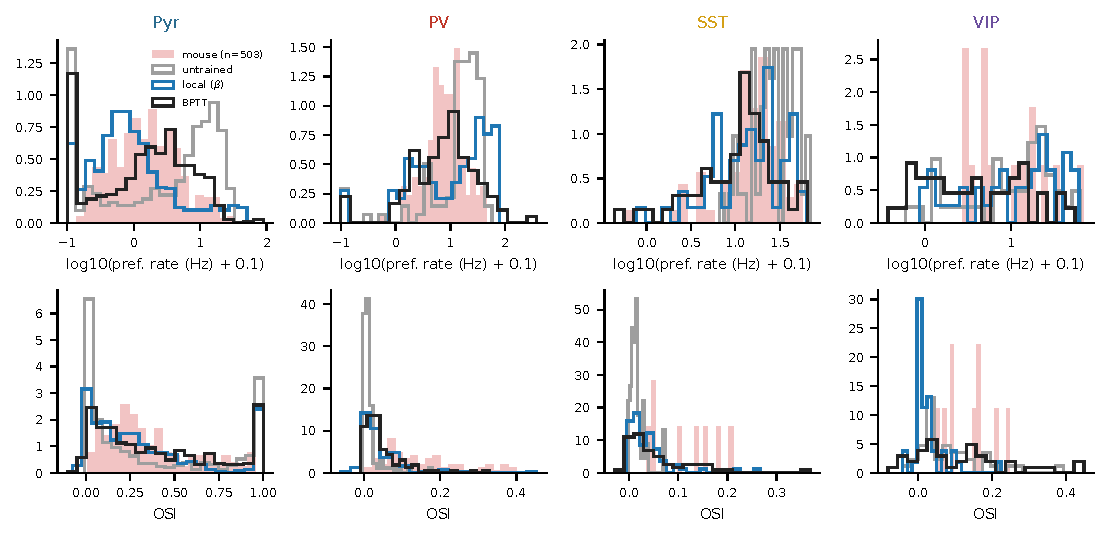
\includegraphics[width=\textwidth]{figures/fig2_tuning.pdf}
\caption{\textbf{Tuning distributions after data-matching training} (one confirmation network).
Shaded: mouse V1 Neuropixels units; lines: model cells of the same type before training and after
local or BPTT training. Top: preferred-direction rate; bottom: OSI of responsive cells.}
\label{fig:tuning}
\end{figure}

\subsection{Reliability-corrected RSA does not depend on the learning rule}
The preregistered primary endpoint is Spearman RSA between model and mouse natural-scene RDMs,
corrected for the reliability of both. It was essentially the same for every condition: 0.38 for
untrained networks, and between 0.36 and 0.39 for every trained network under both objectives
(Fig.~\ref{fig:geometry}a,g). No contrast approached significance; the largest was local vs no
$\beta$ on data matching, $-0.028$, $p=0.10$. Local vs BPTT differed by $-0.005$ [$-0.033$, $0.026$]
(data matching) and $+0.003$ [$-0.001$, $0.008$] (change detection). Together with the untrained
value, this shows that the image-similarity structure the models share with mouse V1 is set by the
fixed front end and the fitted cells, not by how the recurrent synapses were trained.

\begin{figure}[t]\centering
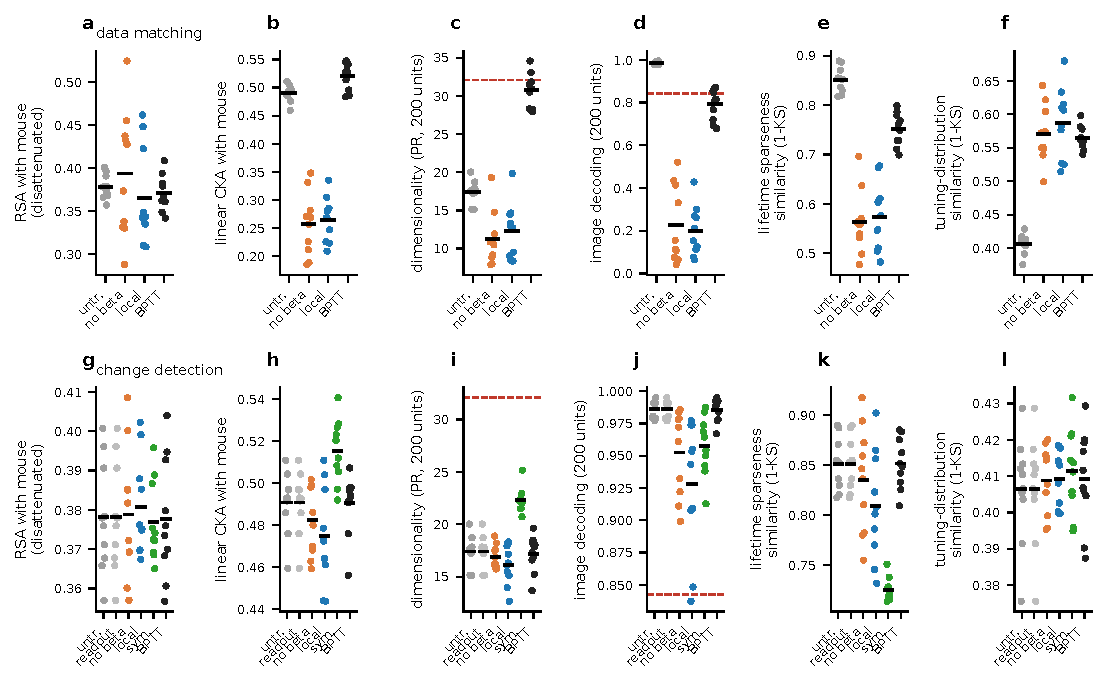
\includegraphics[width=\textwidth]{figures/fig3_geometry.pdf}
\caption{\textbf{Population geometry for 118 held-out natural scenes, compared with mouse V1.}
Each dot is one network (10 per condition); bars show means; red dashed lines show the mouse value.
(a,g) Reliability-corrected RSA (primary endpoint). (b,h) Linear CKA. (c,i) Participation ratio,
200 units. (d,j) Single-repeat image decoding, 200 units. (e,k) Lifetime-sparseness similarity.
(f,l) Mean tuning-distribution similarity. Top: data matching; bottom: change detection.}
\label{fig:geometry}
\end{figure}

\subsection{Data matching: the local rule overshoots into an image-degraded regime}
Under data matching, the secondary measures separated the rules sharply, in the same direction in
all 10 paired networks (Fig.~\ref{fig:geometry}b--e). Each of these contrasts has unadjusted
$p=0.002$, the minimum for 10 pairs. After Holm correction over the full secondary family
($\sim$40 tests) the adjusted value is $p=0.078$.

Compared with BPTT, local-trained networks had:
\begin{itemize}
\item raw RSA with the mouse 0.13 vs 0.32;
\item CKA 0.26 vs 0.52;
\item lower dimensionality: participation ratio 12 vs 31, against 32 in the mouse;
\item much poorer image decoding: 20\% vs 79\%, against 84\% in the mouse;
\item less mouse-like lifetime sparseness: similarity 0.57 vs 0.75.
\end{itemize}
Their natural-scene RDMs were also unreliable across repeats (0.14 vs 0.77). This is why the
reliability-corrected RSA was unchanged while the raw RSA fell.

The cause is visible in the circuit. On average the local rule multiplied the recurrent
magnitudes by a relative change of 87, against 2.5 for BPTT. It also drove PV cells to 43\,Hz
during natural scenes (BPTT 8\,Hz). Removing $\beta$ from the eligibility trace made no detectable
difference to any geometry measure.

\paragraph{At matched performance the rules agree.} Representations along training were related to
the data loss at each checkpoint (Fig.~\ref{fig:traj}a,b). At equal loss the local and BPTT
trajectories coincide. At the loss BPTT reached at its best ($\approx$1.5), local networks (step 200,
loss 1.39) had RSA 0.34 and CKA 0.54, the same as BPTT (0.31--0.34 and 0.51--0.54). The local
networks' geometry collapsed only after they continued past that point, fitting the
grating and gray statistics more closely than BPTT ever did. The divergence is therefore a
property of the solutions the local rule can reach, not a signature of the rule at matched
performance.

\begin{figure}[t]\centering
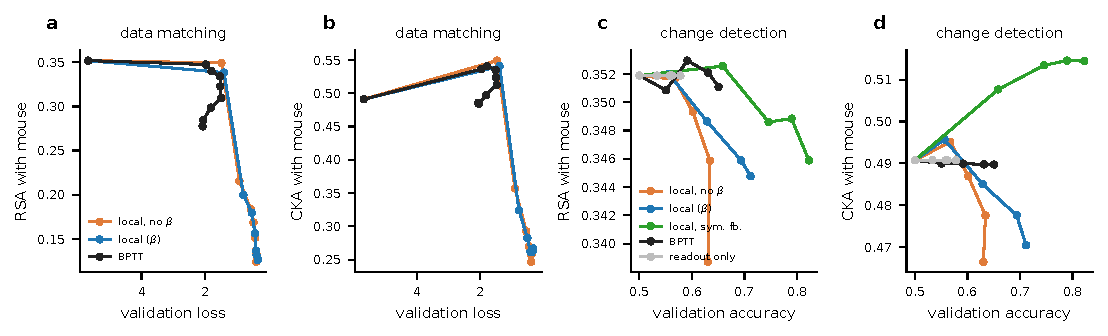
\includegraphics[width=\textwidth]{figures/fig4_trajectory.pdf}
\caption{\textbf{Geometry along training.} Mean RSA (raw) and CKA with mouse V1 at each saved
checkpoint, plotted against that checkpoint's validation value (10 networks per rule). (a,b) Data
matching (loss decreases to the right). (c,d) Change detection (accuracy).}\label{fig:traj}
\end{figure}

\subsection{Change detection: small, rule-specific changes on top of a fixed geometry}
In change detection, the local rule reached higher validation accuracy than BPTT: 0.76 vs 0.68
(readout only 0.62). Symmetric-feedback local reached 0.84. Natural-scene geometry changed little
under every rule: the correlation of each network's RDM with its own untrained RDM was 0.99
(BPTT), 0.92 (local) and 0.94 (symmetric feedback). Two consistent effects appeared, both in 10/10
networks with unadjusted $p=0.002$ (Holm-adjusted $p=0.125$):
\begin{itemize}
\item local learning slightly lowered image decoding (93\% vs 98.5\% for BPTT);
\item local learning with symmetric feedback raised dimensionality (PR 22 vs 16) and CKA with mouse
V1 (0.52 vs 0.47).
\end{itemize}

\begin{figure}[t]\centering
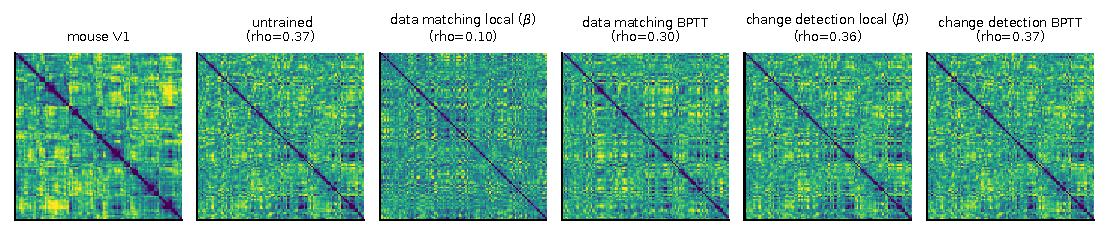
\includegraphics[width=\textwidth]{figures/fig5_rdms.pdf}
\caption{\textbf{Natural-scene RDMs} (one confirmation seed). Images are ordered by hierarchical
clustering of the mouse responses. Titles give the Spearman correlation with the mouse RDM.}
\label{fig:rdms}
\end{figure}

\section{Discussion}

We asked whether training a biologically constrained V1 circuit with a cell-local rule rather than
the exact gradient leaves a measurable trace in its population geometry, and which brings it closer
to mouse V1. Four conclusions follow from the confirmatory data.

\paragraph{The shared image geometry is set before learning.} The reliability-corrected agreement
with mouse V1 on 118 natural scenes was the same for untrained networks and for every learning rule,
under both objectives. In this circuit, what natural images look like to the population is
determined by the front end, the fitted cells and the measured wiring. That is consistent with
models in which V1 selectivity is largely feedforward \citep{lien2018}. It also cautions against
reading RSA agreement as evidence for any particular learning rule. An untrained, well-constrained
circuit already achieves it, so an untrained baseline and reliability correction are essential.

\paragraph{Rules differ in where they can take the circuit.} With matching in-vivo statistics as
the goal, the local rule optimized the trained statistics further than BPTT. It did so by
multiplying recurrent weights roughly 90-fold and driving interneurons hard. This solution
generalized poorly to natural images: dimensionality, decodability and sparseness moved away from
mouse values. BPTT stopped earlier and retained mouse-like dimensionality and decodability.
Crucially, at matched loss the two rules produced the same geometry. The difference is therefore
not an intrinsic signature of local credit assignment but a consequence of which regions of
weight space each rule can reach. Local rules ignore network feedback in their gradient estimates
and can keep pushing in a direction that the exact gradient would correct. This argues for adding
mechanisms that bound such drift, such as weight or rate homeostasis, when local rules are used to
fit data, and for comparing learning rules at matched performance.

\paragraph{On a behavioral task the representation barely moves.} Training change detection on
eight images changed natural-scene geometry little under any rule. The local rule solved the task
better than BPTT at the shared learning rates, and with symmetric feedback it raised
dimensionality towards the mouse value. These effects are small compared with the
mouse--model gap.

\paragraph{The spike-history term.} Unlike in our earlier abstract tasks, removing $\beta$ from the
eligibility trace did not change any geometry measure here. Its importance appears to depend on
whether the task requires credit assignment through the cells' adaptation dynamics.

\paragraph{Relation to the specification's hypotheses.} We did not find that local learning yields
representations ``significantly more'' similar to mouse V1 than BPTT. On the preregistered endpoint
the rules were indistinguishable, and on several secondary measures BPTT was closer to the mouse
under data matching.

\paragraph{Limitations.}
\begin{itemize}
\item \emph{Front end and fixed inputs.} The LGN model and the LGN$\to$V1 weights are simplified
and fixed. Plastic thalamocortical weights would give learning more leverage over geometry.
\item \emph{Rates, not spikes; 20-ms bins.} Fano factors and spike-timing statistics cannot be
compared with the recordings.
\item \emph{Scale and cells.} The circuit has 1{,}000 cells sampled with replacement from about 300
fits, and represents one L2/3-like column without laminar structure.
\item \emph{Learning rates.} Rates were shared across rules and chosen on a small development grid.
BPTT was unstable at the chosen data-matching rate late in training. The change-detection
recurrent rate was not tuned. Matched-performance comparisons address but do not remove this
dependence.
\item \emph{Mouse data.} We used six sessions (627 V1 units) recorded during passive viewing. Units
were pooled across animals into a pseudo-population, and putative cell classes were assigned by
waveform only.
\item \emph{Multiplicity.} The secondary contrasts were consistent across all 10 networks but do not
survive Holm correction over the full secondary family.
\item \emph{Disattenuation.} When a model's RDM reliability is low (0.14 for local data-matching
networks), the corrected RSA is noisy.
\end{itemize}


\section{Methods}\label{sec:methods}

\subsection{Circuit}
Each network contains 1{,}000 cells: 800 pyramidal (Pyr), 100 PV, 60 SST and 40 VIP. The cells
are differentiable generalized firing-rate (GFR) models fitted to Allen Cell Types patch-clamp
recordings \citep{yeung2025gfr}, sampled with replacement within type from a donor-disjoint
cohort. Development used 298 fitted cells and confirmation used a disjoint set of 299 cells; no
donor contributes to both. Each cell has $K=8$ input and spike-history filters (time constants
$\approx$0--2\,s) and a fitted static nonlinearity, simulated at the fitted $\Delta t=20$\,ms:
\begin{equation}
h^{(k)}_{i,t}=(1-d_k)h^{(k)}_{i,t-1}+a_{ik}I_{i,t}+\beta_{ik}r_{i,t-1},\qquad
r_{i,t}=\gamma_i\,\mathrm{ReLU}\big[\tanh\big(\textstyle\sum_d c_{id}^2 x_{i,t}^d\big)\big],
\end{equation}
with $x_{i,t}=(\bar h_{i,t}-b_i)/\sigma_i$. Intrinsic parameters are never trained. A label-free
current sweep sets each cell's isolated baseline to 2\% of its fitted ceiling. The input current is
\begin{equation}
I_{i,t}=I^0_i+S_i\Big(\textstyle\sum_\ell W^{\rm LGN}_{i\ell}(g_{\ell,t}-\bar g^{\rm gray}_\ell)
+\sum_j s_j|W_{ij}|\,r_{j,t-1}/R_0+\xi_{i,t}\Big),
\end{equation}
with Dale signs $s_j$, $R_0=100$\,Hz and Gaussian background noise $\xi$ ($\sigma=0.15$).

\paragraph{Connectivity.} Peak connection probabilities between L2/3 excitatory, PV, SST and
VIP cells were taken from the Allen V1DD electron-microscopy estimates used by
\citet{ito2026} (their \texttt{pmax\_matrix\_v1dd.csv}). Excitatory-to-excitatory probability was
modulated by orientation difference with their like-to-like rule ($\beta=0.5$). Magnitudes are
log-normal ($\sigma_{\log}=0.8$) and scaled by the median 90th-percentile PSP of each pre/post type
pair from the Allen synaptic-physiology survey \citep{campagnola2022}. They are normalized by
in-degree, with inhibitory sources ×2.

\paragraph{Visual input.} Stimuli are rendered on a 48$\times$64 grid (2$^\circ$/pixel). The LGN
front end has ON and OFF centre-surround units (difference of Gaussians, 2$^\circ$/6$^\circ$) on a
stride-2 grid, each with a sustained (40\,ms low-pass) and a transient (20$-$80\,ms band-pass)
channel, rectified around a baseline (3{,}072 units). LGN$\to$V1 weights are fixed. Each Pyr cell
pools ON and OFF subfields of a Gabor template at its preferred orientation and receptive-field
position. Each subfield draws on sustained or transient channels at random, which yields direction
preference \citep{lien2018}. Interneurons receive broader, weaker and mostly untuned input.

\subsection{Objectives}
\emph{Data matching} (following \citealp{ito2026}): one batch has four gray-screen trials and two
trials per direction of an 8-direction drifting grating (0.04\,cpd, 2\,Hz, 80\% contrast), each
500\,ms after 200\,ms of warm-up. For each cell type, the loss is the squared 1-D Wasserstein
distance between model and in-vivo distributions of log spontaneous rate, log preferred-direction
rate, OSI and DSI. OSI and DSI use the form of \citet{ito2026} and are computed only for cells
responding at $\ge$0.5\,Hz. In-vivo targets are the curated Visual Coding Neuropixels units of
\citet{ito2026} \citep{siegle2021}: L2/3 excitatory (503 units) and L2/3 PV (133) cells, and SST (70)
and VIP (16) cells pooled over layers.

\emph{Change detection} follows the structure of the Allen Visual Behavior task: gray, image A for
240\,ms, 500\,ms gray, image B for 240\,ms. The network reports whether B differs from A from the
mean readout of Pyr cells 100--500\,ms after B onset. Images come from a fixed set of eight natural
movie frames, chosen to be maximally distinct, as mice in that task see eight images. A weak
homeostatic term keeps each cell's mean rate near its calibrated baseline. No image used for
evaluation is ever used for training.

\subsection{Learning rules}
Only the recurrent magnitudes $|W_{ij}|$ (fixed mask and sign) and the readout learn. All rules
use Exponentiated Adam \citep{ito2026,cornford2024egd}: $|W|\leftarrow|W|\exp(-\eta\,\hat m/(\sqrt{\hat
v}+\epsilon))$. This update is multiplicative and sign-preserving.

\emph{BPTT} uses the exact gradient through every filter, spike-history loop and recurrent path.

\emph{Local} (e-prop; \citealp{bellec2020eprop}) uses
$\hat g_{ij}=\sum_t L_{i,t}\,\partial r_{i,t}/\partial|W_{ij}|$, where the derivative follows only
cell $i$'s own filters and spike-history loop and treats other cells' activity as given input. We
compute it with automatic differentiation by detaching presynaptic activity in the synaptic input
path. Forward values are unchanged; with no recurrent paths the estimate equals BPTT exactly
(unit test). The learning signal $L_{i,t}$ is the cell's direct error for the data objective. For
change detection it is the readout error broadcast through a fixed random feedback vector.

\emph{Local (no $\beta$)} additionally detaches the spike-history path.

\emph{Readout} keeps the recurrent weights fixed.

\emph{Untrained} is the same circuit before learning.

Every rule used the same learning rates, chosen on the development cohort by validation loss:
$\eta_{\rm rec}=0.015$ for data matching (best for every rule in $\{0.002,0.005,0.015\}$; BPTT was
already unstable late in training at this value, so larger values were not tried) and
$\eta_{\rm rec}=0.005$, $\eta_{\rm out}=0.3$ for change detection (the readout rate was best for every
rule in $\{0.1,0.3,1\}$; the recurrent rate was not tuned). Training ran for 1{,}500 (data) or 800
(change) updates, and the checkpoint with the best validation value was evaluated.

\subsection{Evaluation and comparison with mouse V1}
After training, every network saw:
- the 118 Brain Observatory natural scenes, 240\,ms each, back to back in a new random order on
  each of 10 repeats, as in the recordings \citep{siegle2021,devries2020};
- 2-s drifting gratings in 8 directions;
- 2-s gray screen.

\paragraph{Mouse data.} We used VISp units passing Allen quality criteria (ISI violations
$<0.5$, amplitude cut-off $<0.1$, presence ratio $>0.9$) from the Visual Coding Neuropixels
sessions with the most V1 units. For each unit we took spike counts 0--250\,ms after each of the 50
presentations of each scene. Units were pooled into a pseudo-population; regular- and fast-spiking
units were separated at a 0.4\,ms trough-to-peak waveform duration.

\paragraph{Geometry.}
- \emph{RDM}: 1 minus the Pearson correlation between z-scored population vectors
  \citep{kriegeskorte2008rsa}.
- \emph{RSA}: Spearman correlation between the upper triangles of the model and mouse RDMs. We also
  report a disattenuated version that divides by the square root of the product of the two RDMs'
  Spearman--Brown-corrected split-half (repeat) reliabilities.
- \emph{CKA}: linear CKA \citep{kornblith2019cka} on z-scored image$\times$unit matrices.
- \emph{Dimensionality}: participation ratio of the image-response covariance with 200 units
  subsampled.
- \emph{Lifetime sparseness} \citep{vinje2000}.
- \emph{Image decoding}: nearest-centroid, leave-one-repeat-out, 200 units and 10 repeats for both
  model and mouse.
- \emph{Tuning distributions}: similarity to the in-vivo distributions per cell type (1 minus the
  Kolmogorov--Smirnov statistic).
- \emph{Geometry along training}: to separate learning-rule effects from task performance, we
  recomputed RSA and CKA at every saved checkpoint and related them to that checkpoint's
  validation value.

\paragraph{Statistics.} The unit of analysis is the network seed (10 per condition, paired across
rules). We used exact two-sided sign-flip tests and percentile bootstrap CIs, with Holm correction
within each objective's primary family. The protocol was locked before the confirmation runs
(\texttt{docs/PREREGISTRATION\_v12.md}, \texttt{docs/LOCK\_v12.json}).


\section*{Code and data availability}
All code, configurations, the locked protocol (\texttt{docs/PREREGISTRATION\_v12.md},
\texttt{docs/LOCK\_v12.json}) and per-network results are in the project repository. The fitted
neuron models come from \citet{yeung2025gfr}. Connectivity tables and curated Neuropixels statistics
come from \citet{ito2026}. Neuropixels recordings and natural-scene images are from the Allen
Brain Observatory \citep{siegle2021}.

\bibliographystyle{abbrvnat}
\bibliography{refs,refs_extra}
\end{document}
